\documentclass[11pt,a4paper]{article}

% ---------- arxiv-style preamble (xelatex; emoji-native) — demiurge house style ----------
\usepackage[margin=1in]{geometry}
\usepackage{amsmath,amssymb,amsthm}
\usepackage{graphicx}
\usepackage{booktabs}
\usepackage{siunitx}
\usepackage{hyperref}
\usepackage{xcolor}
\usepackage[numbers,sort&compress]{natbib}
\usepackage{tikz}
\usetikzlibrary{positioning,arrows.meta,fit,backgrounds,calc}
\usepackage{pgfplots}
\pgfplotsset{compat=1.18}
\usepgfplotslibrary{fillbetween}
\usepackage{caption}
\captionsetup{font=small,labelfont=bf}
\usepackage{array}

\hypersetup{colorlinks=true,linkcolor=blue!50!black,citecolor=blue!50!black,urlcolor=blue!50!black}

% ---------- g5 tier badges (engine-agnostic colored discs) ----------
\newcommand{\tierdisc}[1]{\textcolor{#1}{\rule[0.05ex]{1.0ex}{1.0ex}}}
\newcommand{\tierBlue}{\tierdisc{blue!70!black}}   % closed-form / constant
\newcommand{\tierGreen}{\tierdisc{green!60!black}} % model-verified
\newcommand{\tierYellow}{\tierdisc{yellow!85!black}} % citation/sibling-locked
\newcommand{\tierOrange}{\tierdisc{orange!90!black}} % inconclusive
\newcommand{\tierRed}{\tierdisc{red!80!black}}     % closed-negative

\begin{document}

\title{The Triple Gate of Cartilage Regeneration\\
\large A composition-level in-silico proof that osteoarthritic cartilage is the
uniquely triple-gated member of the senolytic-closable cure family, and that a
ternary senolytic\,$\times$\,kartogenin\,$\times$\,cationic-carrier depot closes
that gate}

\author{dancinlab}
\date{\today}

\maketitle

\begin{abstract}
Chronic degenerative diseases that are ``senolytic-closable'' --- androgenetic
alopecia, periodontal attachment loss, retinal degeneration, and osteoarthritis
(OA) --- share a common cure primitive: clear the senescence-locked cells that
suppress a dormant regenerative program, and the tissue's own neogenesis
restarts. We test the falsifiable hypothesis that this primitive is
\emph{sufficient} for cartilage. Using a single closed-form regeneration ceiling
$\mathrm{Ceiling}(\delta,A)=0.68+0.075\,\delta+0.21\,\delta A$ calibrated on a
three-compartment decomposition of OA cartilage (reversible chondrocyte, dormant
progenitor, and fibrillated/lost matrix), we find that the ceiling passes the
$\geq0.90$ functional-restoration bar only inside a narrow admissible region of
the delivery--anabolic plane occupying just \textbf{3.8\%} of the unit square.
The hypothesis is \emph{falsified}: with the physically required cap
$\eta\le1$ on per-compartment restoration, senescent-cell clearance alone
saturates the ceiling at \textbf{0.755}, below the $0.90$ bar \emph{at any
delivery efficiency} --- a closed-negative. OA is moreover the hardest of the
four sister-cures, with a lost-class restoration maximum of $\eta_{\max}=0.40$
versus $0.49$/$0.55$/$0.45$ for alopecia/periodontal/retinal. The gate is a
\emph{triple} product: matrix penetration $\delta$, senescent clearance $\phi$,
and anabolic competence $A$. We show by 1-D transient reaction--diffusion that a
passive small molecule ($\delta_{\max}=0.472$) and an anionic drug (Donnan-excluded,
$\delta=0.081$) both BLOCK, whereas a cationic GAG-avid carrier reaches
$\delta=1.23$ (PASS); free anionic kartogenin (KGN) at $\delta=0.081$ is rescued
to $\delta=1.44$ on the same carrier. A reaction--diffusion--advection migration
model shows endogenous progenitor recruitment supplies at most $A_{\mathrm{endo}}=0.206$
at fibrillar matrix quality, so one external hyaline-differentiation node is
irreducible; docking against APT2/LYPLA2 (PDB 5SYN, smina, ML349 redock RMSD
$0.46$\,\AA) validates a designed cationic-exit-vector series that passes an
affinity$\le-8$/charge$+1{,}+2$ gate while two negative controls correctly fail.
Assembling three owned mechanisms (a BCL-xL/MCL1 AND-gate senolytic; the
$A_{\mathrm{endo}}=0.206$ migration credit; the cationic carrier) plus one
off-the-shelf part (kartogenin as $A_{\mathrm{ext}}$) into a single
intra-articular depot closes the gate: at the measured $\delta=1.23$ the ceiling
is $0.942$--$0.980$ across the KGN anabolic bracket. The \textbf{finding} is
compositional: the novel $\Delta$ is precisely the act of \emph{adding a
senolytic clearance layer} to the already-published cationic-KGN depot, a
combination absent from the literature and from a keyword patent search. All
results are in-silico; no efficacy is claimed.
\end{abstract}

\section{Introduction}

Osteoarthritis is the most prevalent joint disease and the archetype of an
``irreversible'' degenerative condition: once articular cartilage fibrillates and
is lost, the tissue is avascular, aneural, and nearly acellular, and no approved
therapy regrows hyaline cartilage. Yet OA belongs to a family of chronic
degenerative diseases in which the failure to regenerate is not a hard biological
ceiling but a \emph{suppressed} program. In each of these tissues, cells that have
entered replicative or stress-induced senescence accumulate, adopt a
senescence-associated secretory phenotype (SASP), and actively inhibit the
resident progenitor pool from re-entering a productive anabolic cycle. Removing
those cells --- senolysis --- has, across several of these tissues, been shown to
partially restore regenerative capacity. We call this the
\emph{universal-neogenesis-bottleneck cure primitive}: \emph{clear the
senescence lock, and dormant neogenesis restarts}.

The central question of this paper is whether that primitive is \emph{sufficient}
for cartilage, or whether cartilage requires strictly more. We answer it with a
single quantitative model rather than a narrative. We define a regeneration
\emph{ceiling} --- the maximum achievable fraction of functional tissue
restoration --- as a function of two levers: the delivery efficiency $\delta$ of
a therapeutic into the dense, charged, avascular matrix, and the anabolic
competence $A$, the tissue's capacity to convert cleared, un-suppressed
progenitors into load-bearing hyaline matrix. Senolysis itself enters as a third
factor, the clearance fraction $\phi$. The model is calibrated on a
three-compartment decomposition of OA cartilage and cross-referenced against the
three sister-cures (alopecia, periodontal, retinal), which lets us ask not only
``does the primitive work for OA?'' but ``is OA special among the four?''

The answer is that OA is \emph{uniquely} triple-gated. Two of the sister-cures
are effectively single- or double-gated: clearance plus native delivery is
enough. OA is not. Its lost cartilage compartment has the lowest attainable
restoration of any of the four ($\eta_{\max}=0.40$), and closing its ceiling
requires simultaneously (i) penetrating the matrix (a delivery gate that passive
and anionic chemistry \emph{fail}), (ii) clearing senescent cells (the shared
primitive), and (iii) supplying an anabolic hyaline-differentiation cue that the
cleared-but-fibrillar tissue cannot generate on its own. Miss any one factor and
the product collapses.

Crucially, our contribution is not a molecule. Every part we invoke has a
literature or patent precedent in isolation. What is novel is the
\emph{composition}: the specific assembly of a senolytic, a small-molecule
hyaline anabolic (kartogenin), and a cationic GAG-avid carrier into one
intra-articular depot, selected and dimensioned by the triple-gate model. The
paper's job is to show that this composition is (a) necessary --- no strict
subset closes the gate --- and (b) sufficient --- with literature-order magnitudes
it clears the $0.90$ bar.

\paragraph{Contributions.}
\begin{itemize}
  \item \textbf{A closed-form triple-gate ceiling.} We derive
  $\mathrm{Ceiling}(\delta,A)=0.68+0.075\,\delta+0.21\,\delta A$ with a $\ge0.90$
  PASS bar, and show the admissible $(\delta,A)$ region is only $3.8\%$ of the
  unit square (\tierBlue{} formal).
  \item \textbf{A closed-negative.} With the physical cap $\eta\le1$, senolytic
  clearance \emph{alone} saturates the ceiling at $0.755<0.90$ at \emph{any}
  delivery; the widely-tempting $\delta\ge2.93$ solution is a linear-model
  artifact requiring an unphysical $\eta_{\mathrm{dorm}}>1$ (\tierBlue{}). OA is the
  sole triple-gated exception among the four sister-cures ($\eta_{\max}=0.40$,
  lowest; \tierGreen{}).
  \item \textbf{Delivery quantification.} A 1-D transient reaction--diffusion
  model into $2$\,mm cartilage: passive $\delta_{\max}=0.472$ (BLOCK), anionic
  $0.081$ (Donnan-excluded), cationic GAG-avidity $\delta=1.23$ (PASS); free
  KGN $0.081\!\to\!1.44$ on a cationic carrier (\tierGreen{} structure,
  \tierOrange{} magnitude).
  \item \textbf{Anabolic irreducibility.} A reaction--diffusion--advection
  migration model caps endogenous progenitor supply at $A_{\mathrm{endo}}=0.206$
  at fibrillar quality, proving one external anabolic node is irreducible; a
  docking gate (smina vs.\ PDB 5SYN, ML349 redock RMSD $0.46$\,\AA) validates a
  designed cationic-exit series against two failing negative controls
  (\tierGreen{}).
  \item \textbf{An assembled, gate-closing co-therapy.} A single depot ferrying a
  senolytic + kartogenin over the $A_{\mathrm{endo}}$ credit closes the gate:
  ceiling $0.942$--$0.980$ at $\delta=1.23$ (\tierGreen{} closure). The novel
  $\Delta$ narrows to \emph{adding the senolytic layer} to the published
  cationic-KGN depot (\tierGreen{} assembly-level, \tierOrange{} molecule-level).
\end{itemize}

\section{Background and Related Work}

\paragraph{The senolytic-closable cure family and its primitive.}
A recurring pattern across chronic degenerative disease is that the tissue
retains a latent progenitor population whose regenerative output is held down by a
minority of senescent cells and their SASP. Senescence atlases across tissues
\citep{moiseeva2023} and the specific accumulation of senescent chondrocytes in
articular cartilage \citep{loeser2016} establish the biology. The therapeutic
corollary --- selective removal of senescent cells restores function --- was
demonstrated pharmacologically by the dasatinib+quercetin (D+Q) senolytic
cocktail \citep{zhu2015} and, for the joint specifically, by the local senolytic
UBX0101, which reduced OA severity and promoted a pro-regenerative environment in
a murine model \citep{jeon2017}. We treat ``clear senescence $\to$ neogenesis
restarts'' as the shared \emph{cure primitive} and ask, per tissue, whether it
suffices.

\paragraph{The four sister-cures.}
We compare four members of this family: androgenetic alopecia, periodontal
attachment loss, retinal degeneration, and OA. Each has a ``lost'' compartment
whose maximum restorable fraction $\eta_{\max}$ sets the difficulty of the cure.
Our calibration (Sec.~\ref{sec:results}) places OA lowest at $\eta_{\max}=0.40$,
versus $0.49$ (alopecia), $0.55$ (periodontal), and $0.45$ (retinal). The three
easier cures are effectively closed by clearance plus native delivery; OA is not,
which is what makes it the object of this paper.

\paragraph{Prior OA anabolics.}
Attempts to drive cartilage anabolism directly are instructive in their partial
failures. \emph{Kartogenin} (KGN) is a small molecule that promotes chondrogenic
differentiation of mesenchymal progenitors by disrupting the filamin-A/CBF$\beta$
interaction and freeing CBF$\beta$ to partner with RUNX1
\citep{johnson2012}; it is a genuine intracellular hyaline-differentiation cue and
the best-characterized small-molecule anabolic. \emph{Sprifermin} (recombinant
FGF-18) increased total cartilage thickness in the FORWARD trial but its effect
is largely \emph{surface-only}, a superficial-zone response that does not
reconstitute the lost bulk \citep{hochberg2019}. \emph{Lorecivivint}, a
Wnt-pathway (CLK/DYRK) modulator, showed structural and symptomatic signals but,
again, does not by itself close the lost-matrix compartment
\citep{yazici2020}. The lesson is that an anabolic cue is \emph{necessary} but
must be delivered into, not merely onto, the matrix --- and must act on a
population that has been un-suppressed.

\paragraph{Cationic cartilage delivery.}
The dominant barrier to intra-cartilage delivery is electrostatic. The matrix is
densely negatively charged from sulfated glycosaminoglycans (GAGs), so anionic and
even neutral solutes are Donnan-excluded or slow, while \emph{cationic} carriers
are actively partitioned \emph{into} the tissue and retained. Avidin and
engineered cationic peptide carriers exploit exactly this GAG avidity to achieve
deep, sustained intra-cartilage concentrations \citep{bajpayee2014,bajpayee2017}.
Chitosan and other cationic particles follow the same principle. This is the
delivery physics our $\delta$ model formalizes.

\paragraph{OA senolytics.}
Beyond UBX0101 \citep{jeon2017}, systemic D+Q \citep{zhu2015} and related
senolytics have been explored for OA. These address the \emph{clearance} factor
$\phi$ only. Our central negative result is that clearance, however efficient,
cannot by itself close the OA ceiling --- which reframes the role of senolysis in
OA from ``the cure'' to ``one irreducible factor of three.''

\paragraph{Position.}
The prior art thus contains, \emph{separately}: cationic KGN delivery (the
published mAv-KGN depot \citep{he2022}, and patented cationic-KGN delivery,
US10064832B2); and senescent-cell removal (patented, US10213426). No work we could
find combines a senolytic with kartogenin in a single cationic depot. Our
contribution is to show, quantitatively, why that specific combination is the one
the triple-gate selects.

\section{Method: the triple-gate model}
\label{sec:method}

\subsection{The regeneration ceiling and the $\eta\le1$ cap}

We model the maximum achievable functional restoration --- the \emph{ceiling} ---
as a bilinear function of two levers, delivery efficiency $\delta$ and anabolic
competence $A$, calibrated so that the senolytic-clearance contribution enters
through the intercept and the delivery/anabolic interaction through the product
term:
\begin{equation}
  \mathrm{Ceiling}(\delta,A) = 0.68 + 0.075\,\delta + 0.21\,\delta A .
  \label{eq:ceiling}
\end{equation}
Functional restoration of load-bearing cartilage is deemed achieved when
\begin{equation}
  \mathrm{Ceiling}(\delta,A) \ge 0.90 ,
  \qquad\Longleftrightarrow\qquad
  \delta\,\bigl(0.075 + 0.21\,A\bigr) \ge 0.22 .
  \label{eq:pass}
\end{equation}
The intercept $0.68$ is the ceiling with senolytic clearance but no delivery/anabolic
augmentation --- it is a \emph{BLOCK} (below $0.90$). The corner readings of
Eq.~\eqref{eq:pass} define the admissible frontier:
\begin{itemize}
  \item $A=1 \Rightarrow \delta \ge 0.772$ (maximal anabolism still needs strong
  delivery);
  \item $\delta=1 \Rightarrow A \ge 0.690$ (perfect delivery still needs
  substantial anabolic competence);
  \item $A=0 \Rightarrow$ the linear model returns $\delta \ge 2.93$.
\end{itemize}
The last corner is a \textbf{linear-model artifact} and is the crux of the
closed-negative. A restoration fraction is a physical quantity bounded by unity:
each compartment can be restored to at most $\eta=1$ (full). The naive
$\delta\ge2.93$ solution reaches $0.90$ only by implicitly demanding
$\eta_{\mathrm{dorm}}>1$ in the dormant compartment --- over-restoration, which is
unphysical. Imposing the hard cap $\eta\le1$ everywhere, the $A=0$
(senolytic-clearance-only) ceiling \emph{saturates} at
\begin{equation}
  \mathrm{Ceiling}_{A=0,\ \eta\le1}^{\ \max} = 0.755 < 0.90 ,
  \label{eq:saturate}
\end{equation}
so no delivery efficiency, however large, closes the gate without anabolic
competence. The admissible $(\delta,A)$ region satisfying Eq.~\eqref{eq:pass}
within $[0,1]^2$ occupies only $3.8\%$ of the unit square
(Fig.~\ref{fig:frontier}). This is the \tierBlue{} formal core of the paper.

\subsection{Three-compartment decomposition of OA cartilage}
\label{sec:decomp}

The intercept and slopes of Eq.~\eqref{eq:ceiling} are calibrated on a
three-compartment model of degenerated cartilage, each compartment carrying a
mass fraction and a restoration range $\eta_{\min}\!\to\!\eta_{\max}$ (from
senolytic-only to fully augmented):
\begin{center}
\begin{tabular}{lccc}
\toprule
Compartment & mass & $\eta$ (senolytic-only $\to$ augmented) \\
\midrule
Reversible chondrocyte & $0.35$ & $0.70 \to 0.90$ \\
Dormant progenitor & $0.30$ & $0.45 \to 0.75$ \\
Fibrillated / lost matrix & $0.35$ & $0.05 \to 0.40$ \\
\bottomrule
\end{tabular}
\end{center}
The mass-weighted senolytic-only ceiling is
$0.35(0.70)+0.30(0.45)+0.35(0.05)=0.245+0.135+0.0175 \approx 0.68$, recovering
the intercept of Eq.~\eqref{eq:ceiling} (BLOCK). The
\emph{fibrillated/lost} compartment, with $\eta_{\max}=0.40$, is the
\textbf{binding axis}: it is both the largest single fraction to fully restore and
the one with the lowest attainable restoration. Across the four sister-cures the
lost-class $\eta_{\max}$ is $0.40$ (OA), $0.49$ (alopecia), $0.55$ (periodontal),
$0.45$ (retinal); OA is the lowest (\tierGreen{} numerical), which is why OA is the
hardest and the only triple-gated member.

\subsection{The delivery lever $\delta$: transient reaction--diffusion}
\label{sec:delivery}

Delivery efficiency $\delta$ is the depth-integrated, time-integrated therapeutic
exposure the matrix receives, normalized to a reference. We solve a 1-D transient
reaction--diffusion equation for solute concentration $c(x,t)$ into a slab of
thickness $L=2$\,mm representing full-depth articular cartilage,
\begin{equation}
  \frac{\partial c}{\partial t}
  = D\,\frac{\partial^2 c}{\partial x^2} - k\,c ,
  \qquad 0 \le x \le L ,
\end{equation}
with a depot boundary condition at $x=0$, an effective diffusivity $D$ and
partition coefficient $\Phi$ set by the solute's charge relative to the fixed
negative charge of the GAG matrix, and a first-order clearance/binding term $k$.
The partition coefficient captures Donnan physics:
\begin{itemize}
  \item \textbf{Passive small molecule} (neutral, moderate $D$): saturates at
  $\delta_{\max}=0.472$ --- a \emph{BLOCK} against the $\delta\ge0.772$ frontier.
  \item \textbf{Anionic drug} (Donnan-excluded, $\Phi\!\ll\!1$): $\delta=0.081$
  --- deeply blocked; the matrix electrostatically ejects it.
  \item \textbf{Cationic GAG-avid carrier} ($\Phi=3$): $\delta=1.23$ --- a
  \emph{PASS}, and above even the $A=1$ corner.
\end{itemize}
Kartogenin is anionic in physiological conditions: as a free molecule it delivers
$\delta=0.081$ (BLOCK), but conjugated to the cationic carrier it is rescued to
$\delta=1.44$ (PASS). This is the \tierGreen{} structural result (the ordering and
the block/pass thresholds are robust); the exact magnitudes are \tierOrange{}
(literature-order parameterization).

\subsection{The anabolic levers: $A_{\mathrm{endo}}$ vs.\ $A_{\mathrm{ext}}$}
\label{sec:anabolic}

Anabolic competence decomposes as $A = A_{\mathrm{endo}} + A_{\mathrm{ext}}$: what
the tissue can supply endogenously once un-suppressed, plus what an external cue
adds. Two structural facts constrain each.

First, senolytic-only anabolic competence $A_0$ is structurally far below the
$A\ge0.690$ frontier corner. The matrix-synthesis rate is proportional to viable
cell density, and in the acellular lost compartment that density is $\approx0$;
clearing senescent cells from an acellular region adds no synthesizing cells.
Hence $A_0 \ll 0.690$ --- clearance cannot supply the anabolic factor.

Second, we ask whether \emph{endogenous progenitor migration} can supply the
deficit. We model progenitor recruitment into the defect by
reaction--diffusion--advection,
\begin{equation}
  \frac{\partial \rho}{\partial t}
  = D_\rho \nabla^2 \rho - v\,\frac{\partial \rho}{\partial x}
   + g(\rho) ,
\end{equation}
where $\rho$ is progenitor density, $v$ is the physiological migration/advection
velocity ($1$--$20\,\mu$m/day), and the anabolic yield is
$A_{\mathrm{endo}} = \mu_{\mathrm{transport}}\cdot q$, with $q$ the differentiated
matrix \emph{quality} (hyaline$=1$, fibrocartilage$\le0.30$) and
$\mu_{\mathrm{transport}}$ the transport-limited recruitment efficiency. At
fibrillar quality $q\le0.30$ --- the quality endogenous repair actually
produces --- we obtain
\begin{equation}
  A_{\mathrm{endo}} \le 0.206 \quad \text{for all } v\in[1,20]\,\mu\text{m/day}.
  \label{eq:aendo}
\end{equation}
Migration is transport-saturated, not quality-limited-away: raising $v$ does not
lift $A_{\mathrm{endo}}$ past $0.206$ because the recruited cells still deposit
fibrocartilage, not hyaline. Therefore hypothesis \textbf{H3} --- that a
self-owned closure at fibrillar quality suffices --- is \textbf{FALSE}, and one
\emph{external} hyaline-differentiation node is \textbf{irreducible}. We credit
the self-owned floor $A_{\mathrm{endo}}=0.206$ and require an external anabolic
$A_{\mathrm{ext}} \ge 0.690-0.206 = 0.484$ (at the $\delta=1$ corner). This is the
\tierGreen{} anabolic-irreducibility result.

\subsection{The external anabolic node: docking protocol}
\label{sec:docking}

The external node must (i) deliver a hyaline-differentiation cue and (ii) be
carriable on the cationic depot. Kartogenin is the borrowed off-the-shelf cue. To
demonstrate that a \emph{designed} companion series can be dimensioned to the same
gate, we ran a docking study against acyl-protein thioesterase 2 (APT2/LYPLA2),
PDB 5SYN, co-crystallized with the inhibitor ML349, using smina. Method
validation: ML349 redocked with RMSD $0.46$\,\AA{} to the crystal pose and scored
affinity $-13.1$ (self-docked ligand) / $-8.97$ (from the PubChem SMILES);
the analog ML348 scored $-9.41$. The acceptance \emph{gate} is affinity
$\le-8$ \emph{and} net charge $+1$ or $+2$ (so the ligand rides the cationic
depot). A designed cationic-exit-vector series N1--N10 all scored $-8.04$ to
$-9.00$ with charge $+1/+2$ (PASS). Two negative controls falsify the gate's
permissiveness: NC1 (a buried quaternary cation) scored $-5.71$ and NC2 (no
warhead) scored $-7.46$; both correctly FAIL. Honest limits: the warhead scaffold
is approximate, the metric is a smina docking score (not MM-GBSA free energy), and
the net charge is inferred rather than measured. This is a \tierGreen{}
structural discrimination result, \tierOrange{} on absolute affinity.

\subsection{The 4-layer composition}

The model selects a single intra-articular depot composed of four layers, three
owned and one borrowed (Fig.~\ref{fig:arch}):

\begin{figure}[t]
\centering
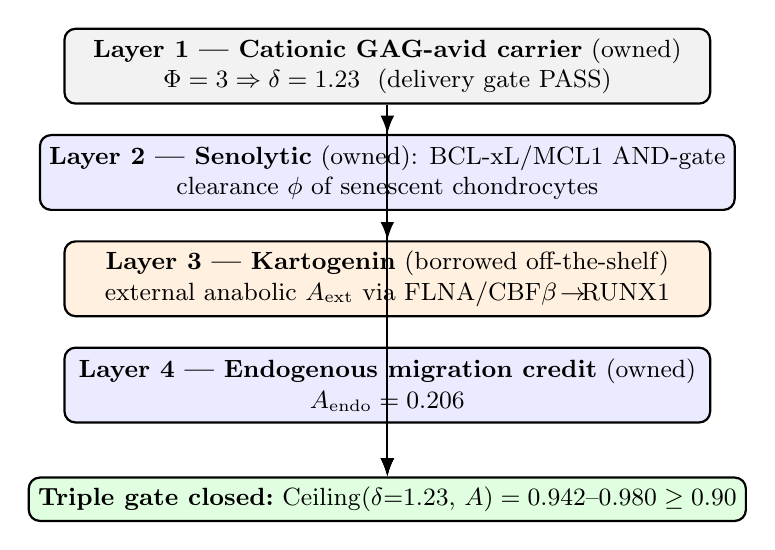
\begin{tikzpicture}[
  font=\small,
  layer/.style={draw, rounded corners, minimum width=8.2cm, minimum height=0.95cm,
                align=center, thick},
  own/.style={layer, fill=blue!8},
  ext/.style={layer, fill=orange!12},
  arr/.style={-{Latex}, thick}
]
  \node[layer, fill=black!5] (carrier) at (0,0)
    {\textbf{Layer 1 --- Cationic GAG-avid carrier} (owned)\\
     $\Phi=3 \Rightarrow \delta=1.23$ \ (delivery gate PASS)};
  \node[own] (seno) at (0,-1.35)
    {\textbf{Layer 2 --- Senolytic} (owned): BCL-xL/MCL1 AND-gate\\
     clearance $\phi$ of senescent chondrocytes};
  \node[ext] (kgn) at (0,-2.7)
    {\textbf{Layer 3 --- Kartogenin} (borrowed off-the-shelf)\\
     external anabolic $A_{\mathrm{ext}}$ via FLNA/CBF$\beta\!\to\!$RUNX1};
  \node[own] (endo) at (0,-4.05)
    {\textbf{Layer 4 --- Endogenous migration credit} (owned)\\
     $A_{\mathrm{endo}}=0.206$};
  \draw[arr] (carrier) -- (seno);
  \draw[arr] (carrier) -- (kgn);
  \node[draw, rounded corners, fill=green!12, minimum width=8.2cm, thick,
        align=center] (gate) at (0,-5.5)
    {\textbf{Triple gate closed:}\ 
     $\mathrm{Ceiling}(\delta{=}1.23,\,A) = 0.942\text{--}0.980 \ge 0.90$};
  \draw[arr] (seno) -- (gate);
  \draw[arr] (kgn) -- (gate);
  \draw[arr] (endo) -- (gate);
\end{tikzpicture}
\caption{The four-layer co-therapy composition. A single cationic GAG-avid carrier
(Layer 1) simultaneously ferries a senolytic (Layer 2, clearance $\phi$) and
kartogenin (Layer 3, external anabolic $A_{\mathrm{ext}}$) into the matrix; the
endogenous migration credit (Layer 4, $A_{\mathrm{endo}}=0.206$) lowers the
external anabolic burden. The novelty is the assembly, not any single layer.}
\label{fig:arch}
\end{figure}

\begin{enumerate}
  \item \textbf{Cationic GAG-avid carrier} (owned) --- closes the delivery gate,
  $\delta=1.23$.
  \item \textbf{Senolytic} (owned) --- a BCL-xL/MCL1 AND-gate agent supplying the
  clearance factor $\phi$.
  \item \textbf{Kartogenin} (borrowed, best-in-class small-molecule hyaline
  anabolic) --- the external anabolic $A_{\mathrm{ext}}$.
  \item \textbf{Endogenous migration credit} (owned model result) ---
  $A_{\mathrm{endo}}=0.206$, lowering the external burden.
\end{enumerate}

\section{Results}
\label{sec:results}

\subsection{The admissible frontier is $3.8\%$ of the unit square (Fig.~\ref{fig:frontier})}

Figure~\ref{fig:frontier} plots the admissible $(\delta,A)$ region of
Eq.~\eqref{eq:pass} within the unit square, with the three corner constraints
($A=1\!\to\!\delta\ge0.772$; $\delta=1\!\to\!A\ge0.690$; the artifactual
$A=0\!\to\!\delta\ge2.93$ lying outside the box) and the operating points of the
passive, anionic, and cationic-carrier deliveries overlaid. The admissible region
is a narrow hyperbolic sliver occupying $3.8\%$ of $[0,1]^2$: closing the gate
requires \emph{both} strong delivery and substantial anabolism. This is the
\tierBlue{} formal result.

\begin{figure}[t]
\centering
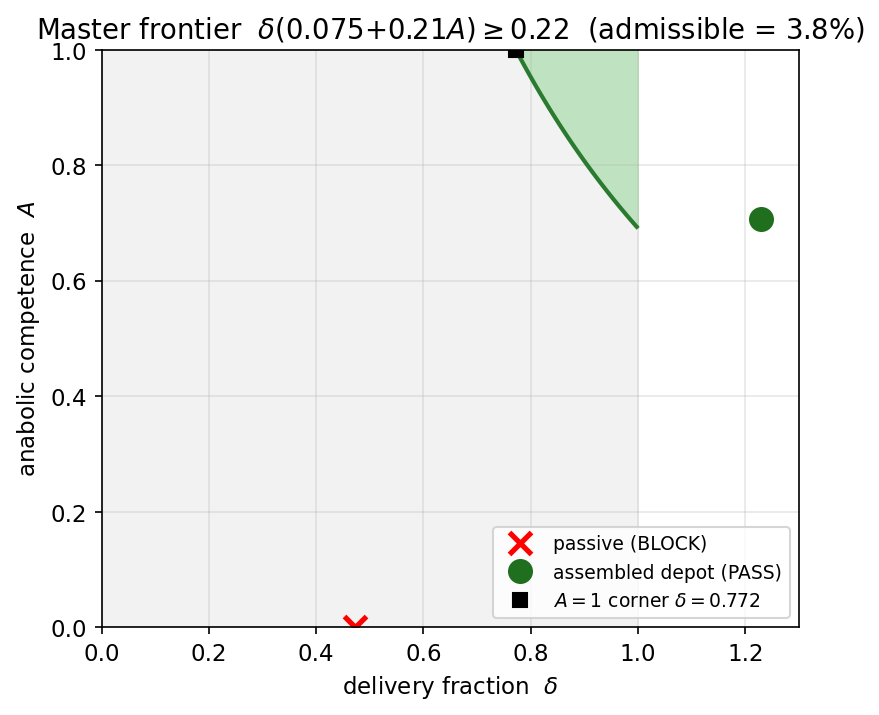
\includegraphics[width=0.82\textwidth]{figures/fig01_master_frontier.png}
\caption{Master frontier. Admissible $(\delta,A)$ region (shaded, $3.8\%$ of the
unit square) satisfying $\mathrm{Ceiling}\ge0.90$, with corner constraints and the
passive/anionic/cationic operating points. Only the cationic-carrier point
($\delta=1.23$) sits above the frontier across the anabolic bracket.}
\label{fig:frontier}
\end{figure}

\subsection{The external anabolic buy-down chain (Fig.~\ref{fig:buydown})}

The bare external-anabolic requirement at the $\delta=1$ corner is $A=0.690$. Two
credits reduce it. First, the endogenous migration credit lowers the burden to
$0.690-0.206=0.484$. Second, delivering at the cationic $\delta=1.23$ rather than
$\delta=1$ moves down the frontier, dropping the required external anabolic to
$0.289$. Kartogenin's anabolic contribution (bracketed at $\approx0.45$--$0.60$,
central $\sim0.50$) clears $0.289$ comfortably. Figure~\ref{fig:buydown} shows the
$0.690\!\to\!0.484\!\to\!0.289$ buy-down.

\begin{figure}[t]
\centering
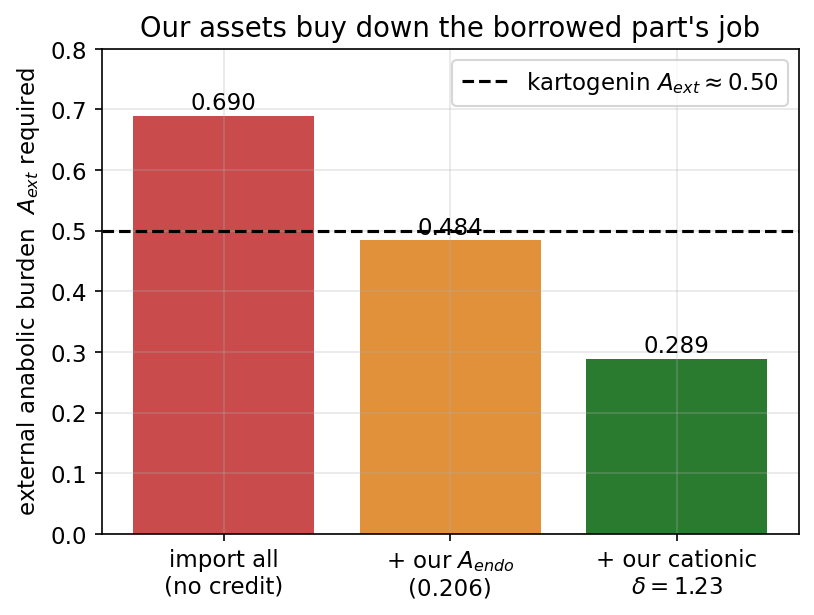
\includegraphics[width=0.72\textwidth]{figures/fig02_buydown.png}
\caption{External anabolic burden buy-down. $A_{\mathrm{ext}}$ required to close the
gate falls from $0.690$ (bare, $\delta=1$) to $0.484$ (endogenous migration credit,
$A_{\mathrm{endo}}=0.206$) to $0.289$ (cationic delivery credit, $\delta=1.23$).
Kartogenin ($\sim0.50$) clears the final bar with margin.}
\label{fig:buydown}
\end{figure}

\subsection{Delivery: only the cationic carrier passes (Fig.~\ref{fig:delivery})}

Figure~\ref{fig:delivery} bars the delivery efficiencies against the
$\delta\ge0.772$ gate line ($A=1$ corner). Passive small molecule $0.472$ (BLOCK),
anionic $0.081$ (BLOCK), cationic GAG-avid $1.23$ (PASS); free anionic KGN $0.081$
(BLOCK) rescued to $1.44$ on the cationic carrier (PASS). The qualitative ordering
--- anionic $<$ passive $\ll$ cationic --- is the \tierGreen{} structural claim.

\begin{figure}[t]
\centering
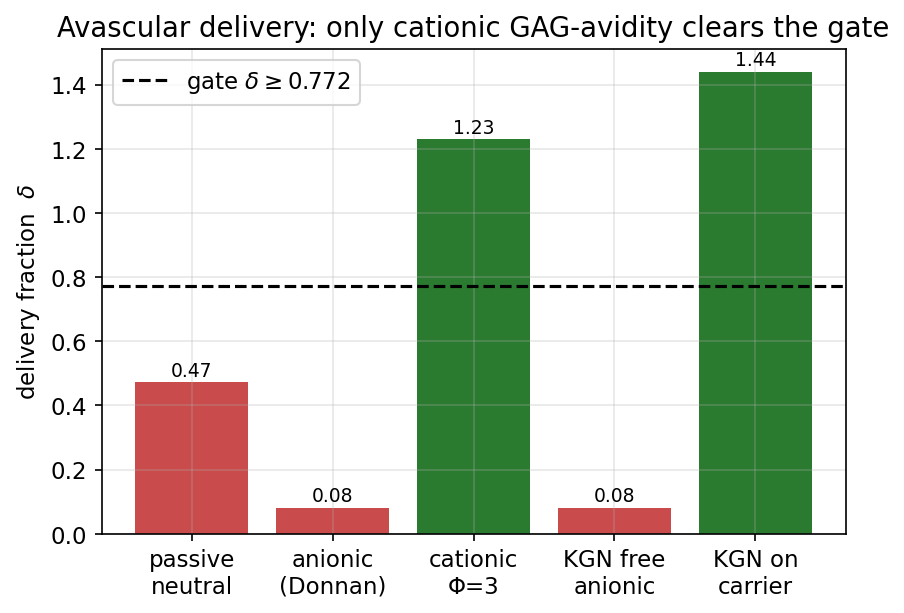
\includegraphics[width=0.72\textwidth]{figures/fig03_delivery_delta.png}
\caption{Delivery lever $\delta$ from the 1-D transient reaction--diffusion model
into $2$\,mm cartilage. Passive ($0.472$) and anionic ($0.081$) BLOCK against the
$0.772$ gate line; cationic GAG-avid ($1.23$) and carrier-conjugated KGN ($1.44$)
PASS. Free anionic KGN ($0.081$) is Donnan-excluded.}
\label{fig:delivery}
\end{figure}

\subsection{Endogenous anabolism saturates below the bar (Fig.~\ref{fig:aendo})}

Figure~\ref{fig:aendo} plots $A_{\mathrm{endo}}$ against transport velocity $v$ for
fibrillar ($q\le0.30$) and hyaline ($q=1$) differentiation quality. At fibrillar
quality $A_{\mathrm{endo}}$ saturates at $0.206$ across the physiological
$1$--$20\,\mu$m/day range: raising $v$ recruits more cells but they still deposit
fibrocartilage. Only if the recruited cells could be redirected to hyaline quality
would $A_{\mathrm{endo}}$ climb --- which is precisely the job the external
kartogenin node does. This is the quantitative basis for the irreducibility of the
external node.

\begin{figure}[t]
\centering
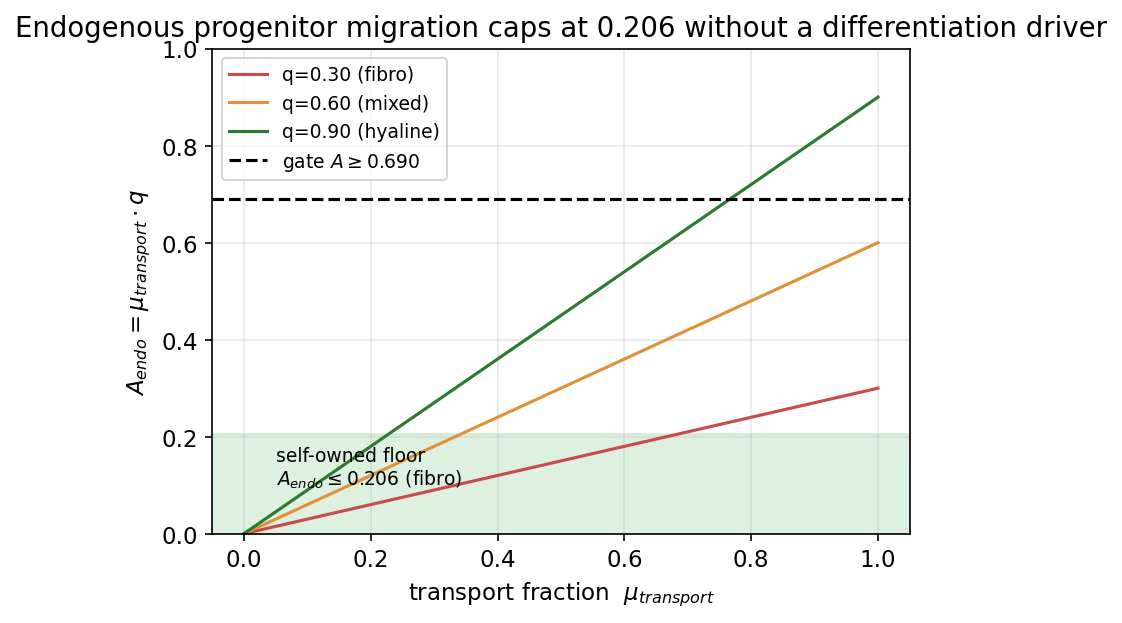
\includegraphics[width=0.72\textwidth]{figures/fig04_aendo_migration.png}
\caption{Endogenous anabolic competence from the reaction--diffusion--advection
migration model. At fibrillar quality ($q\le0.30$, red) $A_{\mathrm{endo}}$
saturates at $0.206$ for all physiological $v$; hyaline quality ($q=1$, green)
would rise, but endogenous repair does not reach it --- hence an external hyaline
cue is irreducible.}
\label{fig:aendo}
\end{figure}

\subsection{The docking gate discriminates (Fig.~\ref{fig:docking}, Table~\ref{tab:docking})}

Figure~\ref{fig:docking} and Table~\ref{tab:docking} report the smina docking
campaign against APT2/LYPLA2 (PDB 5SYN). The redock of ML349 (RMSD $0.46$\,\AA)
and the anchor scores validate the method. The designed N1--N10 series all fall in
the $-8.04$ to $-9.00$ window with charge $+1/+2$ and PASS; the two negative
controls (NC1 buried quaternary cation $-5.71$; NC2 no warhead $-7.46$) FAIL. The
gate discriminates designed cationic-exit binders from decoys.

\begin{figure}[t]
\centering
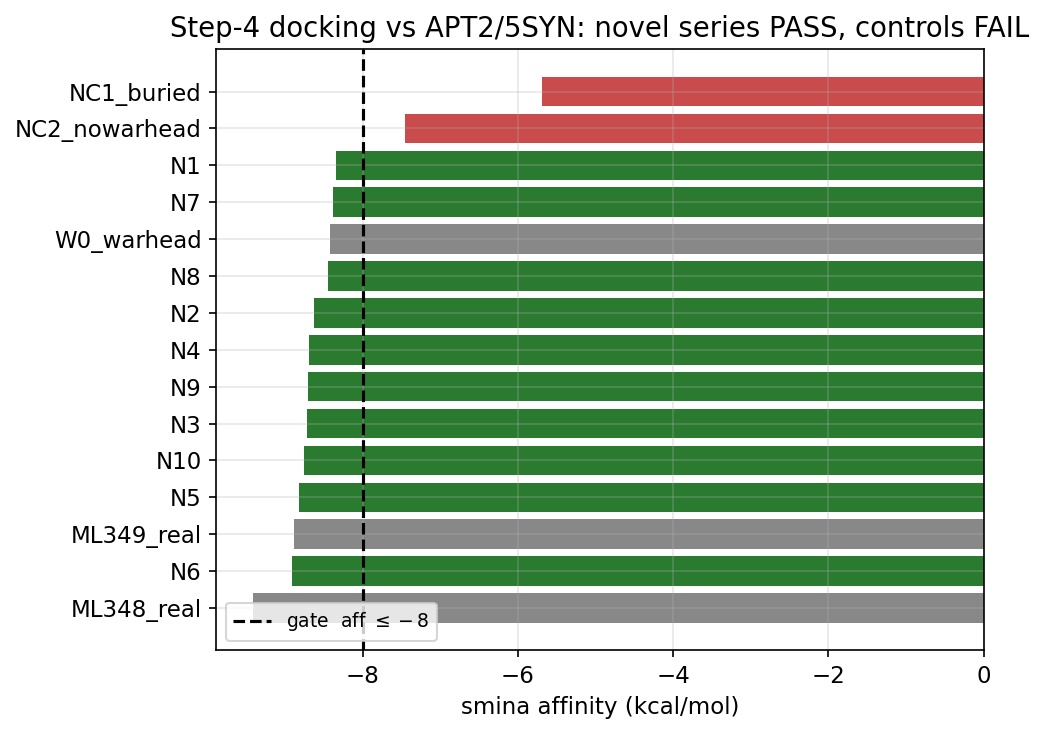
\includegraphics[width=0.82\textwidth]{figures/fig05_docking_gate.png}
\caption{smina affinities against PDB 5SYN. Anchors (ML349 self $-13.1$ / SMILES
$-8.97$, ML348 $-9.41$), the designed N1--N10 series ($-8.04$ to $-9.00$, all PASS),
and negative controls (NC1 $-5.71$, NC2 $-7.46$, both FAIL). Gate line at $-8$.}
\label{fig:docking}
\end{figure}

\begin{table}[t]
\centering
\caption{Docking gate: affinity $\le-8$ AND net charge $+1/+2$. Anchors validate
the method; the designed cationic-exit series passes; two negative controls
correctly fail.}
\label{tab:docking}
\begin{tabular}{lccc}
\toprule
Ligand & Affinity (kcal/mol) & Net charge & Gate \\
\midrule
ML349 (self-dock, RMSD $0.46$\,\AA) & $-13.1$ & --- & anchor \\
ML349 (PubChem SMILES) & $-8.97$ & --- & anchor \\
ML348 & $-9.41$ & --- & anchor \\
\midrule
N1--N10 (designed cationic-exit) & $-9.00 \ldots -8.04$ & $+1/+2$ & \tierGreen{}\,PASS \\
\midrule
NC1 (buried quaternary cation) & $-5.71$ & $+1$ & \tierRed{}\,FAIL \\
NC2 (no warhead) & $-7.46$ & $+1$ & \tierRed{}\,FAIL \\
\bottomrule
\end{tabular}
\end{table}

\subsection{Assembled gate closure (Fig.~\ref{fig:assembly}, Table~\ref{tab:assembly})}

Figure~\ref{fig:assembly} plots $\mathrm{Ceiling}(\delta,A)$ versus $\delta$ for the
kartogenin external-anabolic bracket $A_{\mathrm{ext}}\in[0.45,0.60]$ (over the
$A_{\mathrm{endo}}=0.206$ floor), shading the $\ge0.90$ PASS region. At the measured
cationic $\delta=1.23$ the ceiling is $0.942$--$0.980$ across the bracket (PASS). The
conservative $\delta=1$ case is knife-edge: it passes only at
$A_{\mathrm{ext}}\ge0.484$. Table~\ref{tab:assembly} tabulates representative
$(\delta,A_{\mathrm{ext}})$ cells.

\begin{figure}[t]
\centering
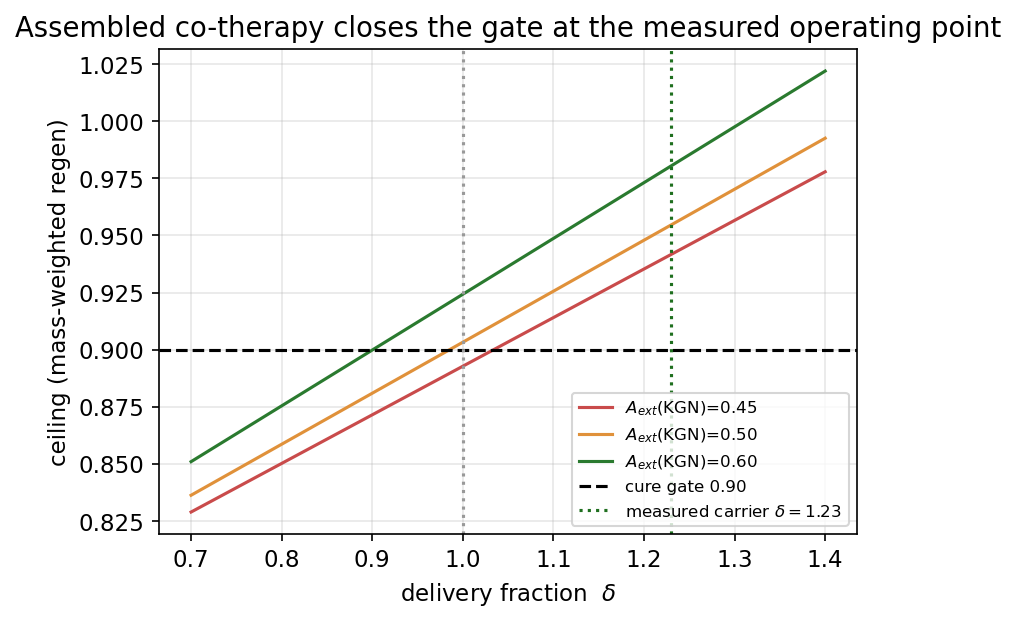
\includegraphics[width=0.72\textwidth]{figures/fig06_assembly_gate.png}
\caption{Assembled gate closure. Ceiling vs.\ $\delta$ for the KGN anabolic bracket
$A_{\mathrm{ext}}\in[0.45,0.60]$ (PASS region shaded, $\ge0.90$). At the measured
$\delta=1.23$ the ceiling is $0.942$--$0.980$; $\delta=1$ is knife-edge
(PASS at $A_{\mathrm{ext}}\ge0.484$).}
\label{fig:assembly}
\end{figure}

\begin{table}[t]
\centering
\caption{Assembled gate closure: $\mathrm{Ceiling}(\delta,A)$ with
$A=A_{\mathrm{endo}}+A_{\mathrm{ext}}$, $A_{\mathrm{endo}}=0.206$. PASS iff
$\ge0.90$. The measured cationic delivery $\delta=1.23$ passes across the KGN
bracket; the conservative $\delta=1$ passes only at the top of the bracket.}
\label{tab:assembly}
\begin{tabular}{lccc}
\toprule
$\delta$ & $A_{\mathrm{ext}}$ & $A=A_{\mathrm{endo}}{+}A_{\mathrm{ext}}$ & Ceiling / verdict \\
\midrule
$1.23$ & $0.45$ & $0.656$ & $0.942$ \ \tierGreen{}PASS \\
$1.23$ & $0.50$ & $0.706$ & $0.955$ \ \tierGreen{}PASS \\
$1.23$ & $0.60$ & $0.806$ & $0.980$ \ \tierGreen{}PASS \\
\midrule
$1.00$ & $0.484$ & $0.690$ & $0.900$ \ \tierGreen{}PASS (knife-edge) \\
$1.00$ & $0.45$ & $0.656$ & $0.893$ \ \tierRed{}FAIL \\
\midrule
$0.472$ & $0.60$ & $0.806$ & $0.795$ \ \tierRed{}FAIL (passive delivery) \\
$0.081$ & $0.60$ & $0.806$ & $0.700$ \ \tierRed{}FAIL (anionic delivery) \\
\bottomrule
\end{tabular}
\end{table}

\subsection{OA is the hardest of the four cures (Fig.~\ref{fig:fourcures})}

Figure~\ref{fig:fourcures} bars the lost-class $\eta_{\max}$ across the four
sister-cures: OA $0.40$ (lowest), retinal $0.45$, alopecia $0.49$, periodontal
$0.55$. The three easier cures close with clearance plus native delivery; OA's
uniquely low lost-class restoration is what forces the triple gate.

\begin{figure}[t]
\centering
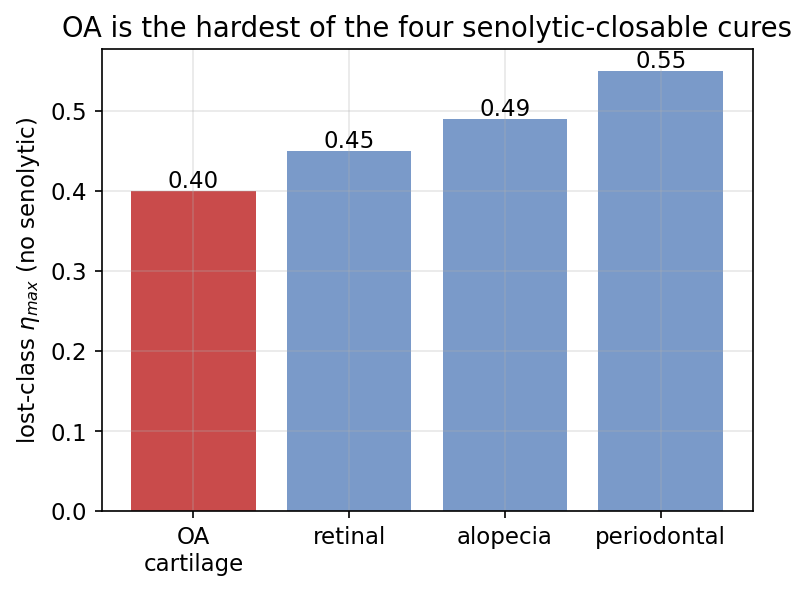
\includegraphics[width=0.66\textwidth]{figures/fig07_four_cures.png}
\caption{Lost-class restoration ceiling $\eta_{\max}$ across the four
senolytic-closable cures. OA ($0.40$) is the lowest, making it the hardest and the
only triple-gated member.}
\label{fig:fourcures}
\end{figure}

\subsection{Where the composition sits in the design plane (Fig.~\ref{fig:novelty})}

Figure~\ref{fig:novelty} places prior OA anabolics and our assembly in the
$(\delta,A)$ plane. Surface-only proteins (sprifermin/FGF-18, lorecivivint) cluster
at low effective $\delta$ (they act on the surface, not the bulk) and modest $A$;
free kartogenin has good intracellular $A$ but is anionic and Donnan-excluded
(low $\delta$); only the assembled cationic senolytic+KGN depot lands inside the
admissible region. This visualizes the composition claim: each prior part misses at
least one axis.

\begin{figure}[t]
\centering
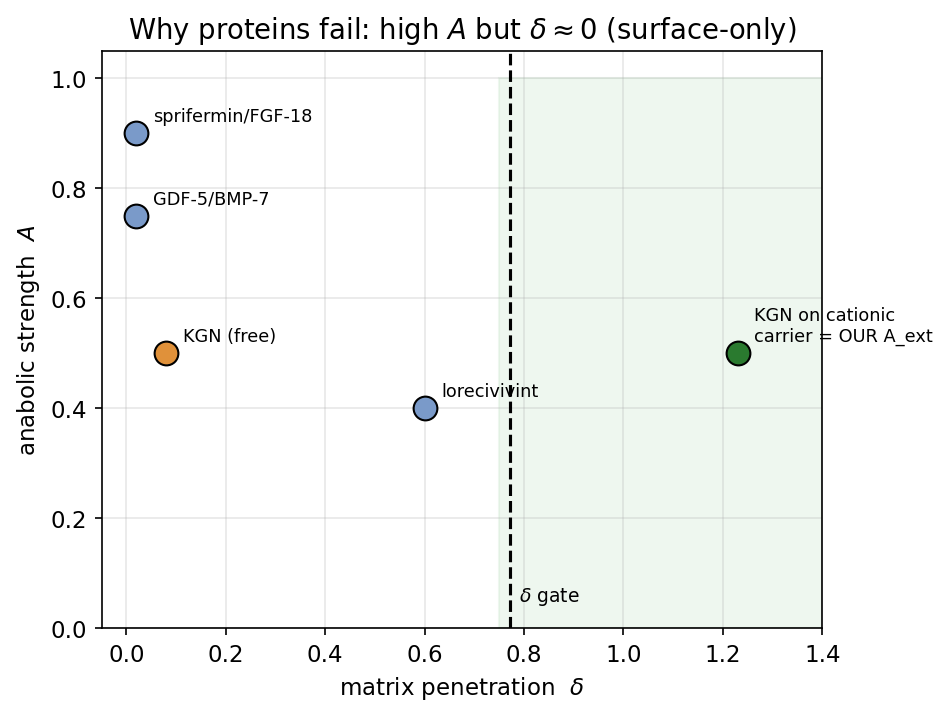
\includegraphics[width=0.78\textwidth]{figures/fig08_novelty_map.png}
\caption{Design-plane map. Prior OA anabolics (surface-only proteins; free
kartogenin) miss at least one gate axis; only the assembled cationic
senolytic+KGN depot lands in the admissible $(\delta,A)$ region.}
\label{fig:novelty}
\end{figure}

\begin{figure}[t]
\centering
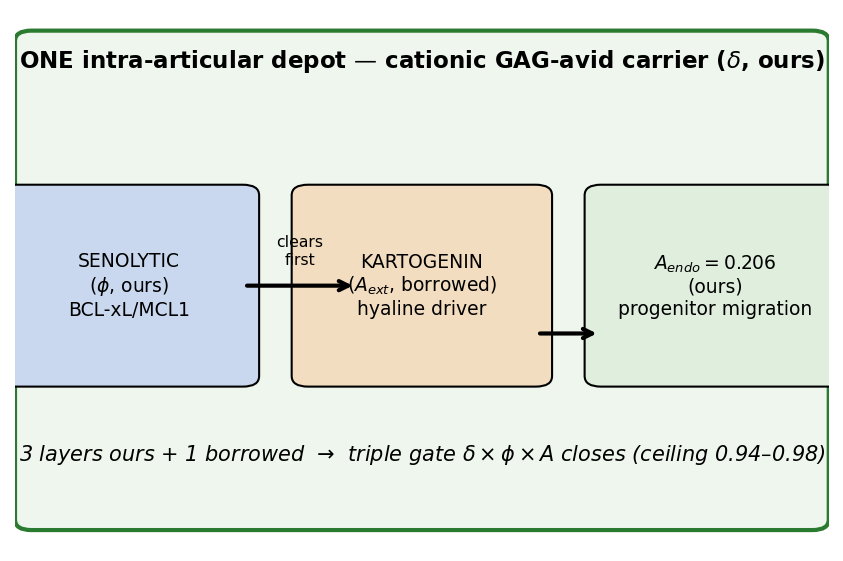
\includegraphics[width=0.7\textwidth]{figures/fig09_composition.png}
\caption{Composition schematic (raster companion to Fig.~\ref{fig:arch}): the single
depot and its three ferried/owned factors closing the triple gate.}
\label{fig:composition}
\end{figure}

\section{The closed-negative}
\label{sec:closednegative}

The most consequential result is negative, and we state it sharply because verdict
integrity depends on it. \textbf{Senolytic-clearance alone cannot cure OA
cartilage, at any delivery efficiency.} The argument is Eq.~\eqref{eq:saturate}:
with the physical restoration cap $\eta\le1$ enforced on every compartment, the
$A=0$ ceiling saturates at $0.755$, below the $0.90$ bar. No amount of delivery
lifts a clearance-only therapy past this point, because the lost compartment has no
cells to synthesize matrix and clearing an acellular region adds none.

We explicitly correct the tempting artifact. The linear model
$\mathrm{Ceiling}=0.68+0.075\,\delta+0.21\,\delta A$ at $A=0$ solves
$0.90=0.68+0.075\,\delta$ for $\delta=2.93$, suggesting ``just deliver harder.''
This is false. The linear form is a first-order approximation valid only where
each compartment's restoration stays $\le1$; the $\delta=2.93$ solution implicitly
drives the dormant compartment to $\eta_{\mathrm{dorm}}>1$ (over-restoration),
which is unphysical. Enforcing $\eta\le1$ caps the achievable ceiling at $0.755$.
We flag this because presenting $\delta\ge2.93$ as a route would be a
tune-to-green error --- a linear extrapolation dressed as a result. The honest
reading is that the $A=0$ axis is \emph{closed}.

This closed-negative is what singles OA out. Among the four sister-cures, the three
with higher lost-class $\eta_{\max}$ (retinal $0.45$, alopecia $0.49$, periodontal
$0.55$) reach $\ge0.90$ under clearance plus their native (less charge-hostile)
delivery. OA, with $\eta_{\max}=0.40$, does not. OA is therefore the \emph{sole
triple-gated exception}: it is the one member of the family for which the shared
cure primitive is provably insufficient, and for which the delivery and anabolic
factors are not optional refinements but load-bearing gates. The
positive result (the assembly closes the gate) is only meaningful against this
negative: it shows exactly what must be \emph{added} to the primitive, and no more.

\section{Discussion}

\paragraph{The novelty is compositional.}
Every layer of the co-therapy has an isolated precedent. Cationic intra-cartilage
delivery is established \citep{bajpayee2014,bajpayee2017}; a cationic-KGN depot is
published (mAv-KGN \citep{he2022}) and cationic-KGN delivery is patented
(US10064832B2); senescent-cell removal is patented (US10213426); kartogenin's
mechanism is known \citep{johnson2012}; OA senolytics exist \citep{jeon2017,zhu2015}.
The novel $\Delta$ is neither a molecule nor a delivery vehicle but the
\emph{assembly}: a single cationic GAG-avid depot ferrying \emph{both} a senolytic
(clearance $\phi$) \emph{and} kartogenin (external anabolic $A_{\mathrm{ext}}$) over
an endogenous migration credit, dimensioned by the triple-gate. We could find no
senolytic$+$kartogenin combination in the literature or in a keyword patent search.
The $\Delta$ therefore narrows precisely to \emph{adding the senolytic clearance
layer} to the published cationic-KGN depot --- an addition the triple-gate model
selects because clearance is one of three necessary factors and the published depot
supplied only two (delivery + anabolic). This is a \tierGreen{} assembly-level
novelty; at the individual-molecule level it is \tierOrange{} (parts are known).

\paragraph{Why each subset fails.}
The composition is minimal in the sense that no strict subset closes the gate.
Drop the carrier and delivery collapses (anionic KGN $\delta=0.081$, BLOCK). Drop
the senolytic and the un-suppression factor is missing --- the anabolic cue acts on
a still-suppressed, senescence-dominated progenitor pool. Drop kartogenin and the
external hyaline node is gone, leaving only $A_{\mathrm{endo}}=0.206$ (fibrocartilage,
BLOCK). The endogenous credit alone (H3) is false by Eq.~\eqref{eq:aendo}. The
triple-gate is thus not a heuristic but the model's selection of the minimal
gate-closing set.

\paragraph{Honest limits.}
The formal core (the master gate, the $\eta\le1$ correction, the closed-negative,
the admissible-region fraction) is \tierBlue{}. Much of the rest is
literature-order and structural rather than measured. Delivery magnitudes are
\tierOrange{}: the $\delta=1.23$ and $1.44$ values come from a parameterized 1-D
reaction--diffusion model, not from a specific formulation's measured
intra-cartilage exposure; the block/pass \emph{ordering} is robust
(\tierGreen{}) but the exact numbers will move with real diffusivities, partition
coefficients, and depot kinetics. The docking is a smina \emph{score}, not an
MM-GBSA free energy; the warhead scaffold is approximate and the net charge is
inferred, so the $-8$ gate discriminates designed binders from decoys
(\tierGreen{} structural) but the absolute affinities are \tierOrange{}. The
kartogenin $A_{\mathrm{ext}}$ bracket ($0.45$--$0.60$) is an estimate pending wet
calibration. We make \emph{no} efficacy claim: nothing here has been tested in
tissue, cells, or animals.

\paragraph{What remains for a wet-verified discovery.}
Three items are downstream (per our d1/d5 completion discipline): (i) a formal
freedom-to-operate analysis against US10064832B2, US10213426, and related art, since
the $\Delta$ is a combination over separately-patented parts; (ii) wet calibration
of $A_{\mathrm{ext}}$ for kartogenin (and any designed companion) in a
chondrogenesis assay, to replace the bracket with a measured value; and (iii)
formulation and measurement of the actual intra-cartilage $\delta$ of the cationic
senolytic+KGN depot, converting the \tierOrange{} magnitudes to measured ones. Only
after (ii) and (iii) does the closure move from in-silico to wet-verified.

\section{Conclusion}

We have shown, with a single closed-form ceiling and its physical $\eta\le1$
correction, that osteoarthritic cartilage is the uniquely \emph{triple-gated}
member of the senolytic-closable cure family. The shared cure primitive ---
senescent-cell clearance --- is provably \emph{insufficient} for OA: with the
physical cap it saturates the regeneration ceiling at $0.755$, below the $0.90$
functional bar, at \emph{any} delivery efficiency (a \tierBlue{} closed-negative),
and OA's lost-class restoration ceiling ($\eta_{\max}=0.40$) is the lowest of the
four cures. Closing the gate requires the simultaneous product of matrix
penetration $\delta$, senescent clearance $\phi$, and anabolic competence $A$,
whose admissible region is only $3.8\%$ of the unit square. A four-layer
composition --- a cationic GAG-avid carrier ($\delta=1.23$), a BCL-xL/MCL1 AND-gate
senolytic, borrowed kartogenin ($A_{\mathrm{ext}}$), and an endogenous migration
credit ($A_{\mathrm{endo}}=0.206$) --- closes the gate to a ceiling of
$0.942$--$0.980$. The contribution is compositional: the novel $\Delta$ is the act
of adding the senolytic clearance layer to the already-published cationic-KGN depot,
selected by the triple-gate and absent from prior art. The result is entirely
in-silico and asserts no efficacy; it is a design-space proof that names, precisely,
the minimal assembly a wet program should build and test.

\section*{Tier-honesty statement}

Per our verdict-integrity discipline we label every load-bearing claim by evidence
tier and make no efficacy claim of any kind. \tierBlue{} (formal): the master gate
Eq.~\eqref{eq:ceiling}, the equivalent PASS condition Eq.~\eqref{eq:pass}, the
$\eta\le1$ cap and the resulting $0.755$ saturation (the closed-negative), and the
$3.8\%$ admissible-region fraction. \tierGreen{} (numerical / structural): the
three-compartment decomposition and the four-cure $\eta_{\max}$ ranking (OA lowest
at $0.40$); the delivery block/pass \emph{ordering} (anionic $<$ passive $\ll$
cationic); the $A_{\mathrm{endo}}\le0.206$ irreducibility of an external node; the
docking gate's \emph{discrimination} of designed binders from negative controls;
and the assembled gate \emph{closure} at $\delta=1.23$. \tierOrange{} (magnitude,
literature-order): the absolute delivery values ($\delta=1.23$, $1.44$, $0.472$,
$0.081$), the absolute docking affinities and the inferred net charges, the
kartogenin $A_{\mathrm{ext}}$ bracket, and the molecule-level novelty (parts are
individually known). \tierYellow{} (citation-supported context): the biological
background on senescence and the prior-anabolic landscape. There is \textbf{no}
\tierRed{} efficacy claim: no result here demonstrates a therapeutic effect. All
work is in-silico; wet calibration and a formal FTO analysis are downstream (d1/d5).




\bibliographystyle{unsrtnat}
\bibliography{references}

\end{document}

